\documentclass[9pt,twocolumn,twoside,]{pnas-new}

% Use the lineno option to display guide line numbers if required.
% Note that the use of elements such as single-column equations
% may affect the guide line number alignment.


\usepackage[T1]{fontenc}
\usepackage[utf8]{inputenc}

% tightlist command for lists without linebreak
\providecommand{\tightlist}{%
  \setlength{\itemsep}{0pt}\setlength{\parskip}{0pt}}


% Pandoc citation processing
\newlength{\cslhangindent}
\setlength{\cslhangindent}{1.5em}
\newlength{\csllabelwidth}
\setlength{\csllabelwidth}{3em}
\newlength{\cslentryspacingunit} % times entry-spacing
\setlength{\cslentryspacingunit}{\parskip}
% for Pandoc 2.8 to 2.10.1
\newenvironment{cslreferences}%
  {}%
  {\par}
% For Pandoc 2.11+
\newenvironment{CSLReferences}[2] % #1 hanging-ident, #2 entry spacing
 {% don't indent paragraphs
  \setlength{\parindent}{0pt}
  % turn on hanging indent if param 1 is 1
  \ifodd #1
  \let\oldpar\par
  \def\par{\hangindent=\cslhangindent\oldpar}
  \fi
  % set entry spacing
  \setlength{\parskip}{#2\cslentryspacingunit}
 }%
 {}
\usepackage{calc}
\newcommand{\CSLBlock}[1]{#1\hfill\break}
\newcommand{\CSLLeftMargin}[1]{\parbox[t]{\csllabelwidth}{#1}}
\newcommand{\CSLRightInline}[1]{\parbox[t]{\linewidth - \csllabelwidth}{#1}\break}
\newcommand{\CSLIndent}[1]{\hspace{\cslhangindent}#1}


\templatetype{pnasresearcharticle}  % Choose template

\title{Distribution et Abondance des Macroinvertébrés Benthiques en
Fonction des Paramètres Fluviaux au Québec : Une Étude Écologique}

\author[a,1,2]{Alexis Rompré}
\author[a,b]{Gabin Jouen}
\author[b,1,2]{Justin Gagnon}

  \affil[a]{Université de Sherbrooke, Department de Biologie, Bd de
l'Université, Sherbrooke, Québec, J1K 2R1}


% Please give the surname of the lead author for the running footer
\leadauthor{Rompré}

% Please add here a significance statement to explain the relevance of your work
\significancestatement{}


\authorcontributions{}



\correspondingauthor{\textsuperscript{2} To whom correspondence should
be addressed. E-mail:
\href{mailto:alexis.rompre@usherbrooke.ca}{\nolinkurl{alexis.rompre@usherbrooke.ca}}}

% Keywords are not mandatory, but authors are strongly encouraged to provide them. If provided, please include two to five keywords, separated by the pipe symbol, e.g:


\begin{abstract}
Dans cette étude, le ministère de l'Environnement du Québec a analysé la
santé écologique des rivières en mesurant la distribution et l'abondance
des macroinvertébrés benthiques. Les prélèvements effectués ont permis
d'examiner l'impact de variables comme la largeur de la rivière, la
profondeur, la vitesse du courant, la transparence et la température de
l'eau sur ces communautés. Les résultats révèlent qu'aucune corrélation
significative n'est observée entre la largeur, la profondeur et la
vitesse du courant avec l'abondance benthique. Toutefois, la température
de l'eau montre une légère influence positive. Des corrélations
importantes existent entre la profondeur et la largeur des rivières, et
entre ces paramètres et la température, indiquant que des rivières plus
larges et plus profondes ont tendance à être plus chaudes. La
transparence de l'eau affecte également l'abondance du benthos, avec des
niveaux plus élevés dans les eaux moyennement transparentes. Cette
recherche éclaire les dynamiques fluviales et fournit des données
essentielles pour la gestion des ressources aquatiques au Québec,
nécessitant des analyses plus approfondies pour comprendre les
interactions complexes des écosystèmes aquatiques.
\end{abstract}

\dates{This manuscript was compiled on \today}
\doi{\url{www.pnas.org/cgi/doi/10.1073/pnas.XXXXXXXXXX}}

\begin{document}

% Optional adjustment to line up main text (after abstract) of first page with line numbers, when using both lineno and twocolumn options.
% You should only change this length when you've finalised the article contents.
\verticaladjustment{-2pt}



\maketitle
\thispagestyle{firststyle}
\ifthenelse{\boolean{shortarticle}}{\ifthenelse{\boolean{singlecolumn}}{\abscontentformatted}{\abscontent}}{}

% If your first paragraph (i.e. with the \dropcap) contains a list environment (quote, quotation, theorem, definition, enumerate, itemize...), the line after the list may have some extra indentation. If this is the case, add \parshape=0 to the end of the list environment.

\acknow{Please include your acknowledgments here, set in a single
paragraph. Please do not include any acknowledgments in the Supporting
Information, or anywhere else in the manuscript.}

\hypertarget{Introduction}{%
\subsection*{Introduction}\label{Introduction}}
\addcontentsline{toc}{subsection}{Introduction}

Dans le cadre des efforts continus pour comprendre et préserver la
qualité des écosystèmes aquatiques au Québec, le ministère de
l'Environnement, de la Lutte contre les Changements Climatiques, de la
Faune et des Parcs (MELCCFP) a entrepris une série d'inventaires du
benthos. Ces inventaires fournissent des données précieuses sur la
distribution et l'abondance des macroinvertébrés benthiques, des
indicateurs clés de la santé écologique des rivières. Utilisant un filet
à mailles fines (D-net), les équipes du MELCCFP réalisent des
prélèvements standardisés sur un effort d'échantillonnage de 3m²,
effectuant trois passages par site pour maximiser la représentativité
des données. Les échantillons récoltés sont ensuite analysés en
laboratoire. Sur des plateaux de tri, les espèces sont identifiées et
dénombrées, bien que seulement une fraction de chaque échantillon soit
identifiée pour estimer l'abondance globale. Ces informations sont
ensuite reliées à divers paramètres physico-chimiques des sites
d'échantillonnage, tels que la largeur et la profondeur de la rivière,
la vitesse du courant, la transparence et la température de l'eau. Cette
étude scientifique vise à analyser comment ces variables influencent la
distribution et la densité des communautés benthiques. Les résultats de
cette recherche fourniront non seulement une meilleure compréhension des
écosystèmes fluviaux du Québec mais aussi des données essentielles pour
la gestion durable et la conservation des ressources aquatiques.

\hypertarget{Muxe9thode}{%
\subsection*{Méthode}\label{Muxe9thode}}
\addcontentsline{toc}{subsection}{Méthode}

Dans le cadre de notre étude sur l'abondance des macroinvertébrés
benthiques des rivières québécoises, nous avons exploité une base de
données existante fournie par le MELCCFP. Après avoir procédé à un
nettoyage et à une validation rigoureuse des données, nous avons utilisé
une combinaison d'outils et de techniques pour analyser et présenter nos
résultats. Le processus a commencé par le nettoyage des données
écologiques pour éliminer les erreurs et les incohérences, suivi de leur
validation pour assurer l'exactitude et la fiabilité des informations.
Les données nettoyées ont été entreposées dans une base de données SQL,
gérée avec RSQLite pour faciliter la manipulation des données dans
l'environnement RStudio. Pour garantir la reproductibilité de notre
recherche, nous avons utilisé Git pour le versionnage du code.
L'automatisation des scripts d'analyse a été réalisée avec le package «
targets » dans R, permettant une mise à jour efficace et une exécution
systématique des analyses. La visualisation des données a joué un rôle
crucial, utilisant des techniques de conception graphique avancées pour
illustrer clairement les résultats. Enfin, la communication des
découvertes scientifiques a été formalisée à travers des rapports
détaillés en RMarkdown, combinant code, résultats et interprétations
pour une diffusion transparente et accessible des résultats de la
recherche.

\hypertarget{Ruxe9sultats}{%
\subsection*{Résultats}\label{Ruxe9sultats}}
\addcontentsline{toc}{subsection}{Résultats}

La largeur, la profondeur et la vitesse du courant de la rivière liée à
l'abondance totale du benthos, ont montré, respectivement un coefficient
de corrélation non significatif de -0,026, 0.048 et 0.011, nous
empêchant donc d'émettre des conclusions entre ces paramètres et
l'abondance du benthos. Toutefois, la température de l'eau des rivières
montre une corrélation significative légèrement positive (0.073),
suggérant une influence minime de ce paramètre sur l'abondance totale du
benthos. Il est intéressant de constater que des corrélations positives
significatives sont observées entre la profondeur et la largeur des
rivières (0.219), la largeur des rivières et la température de l'eau
(0.290), indiquant que les rivières plus larges et plus profondes
peuvent avoir des températures plus élevées. Mais aussi entre la
température de l'eau et la vitesse du courant des rivières (0,332) et
entre la profondeur et la vitesse du courant des rivières (0,442).

La figure 2 suggère qu'il y a des variations dans l'abondance des
organismes benthiques entre les différentes classes de transparence. Sur
une échelle logarithmique, l'abondance tend à être plus élevée dans les
cours d'eau à transparence élevée et moyenne qu'à transparence faible,
mais avec une étendue des données notables pour la classe « élevée ».
Nous avons donc fait un test de Tukey, qui a révélé uniquement une
différence significative dans l'abondance totale entre les groupes de
transparence moyenne et faible.

La figure 3 illustré ci-dessus présente une régression linéaire (ligne
bleue) entre la vitesse moyenne du courant (m/s) et la température
moyenne de l'eau (°C). Celle-ci montre une relation significative entre
les deux attributs (p-value = 3,064 x 10-11***) ainsi qu'un R2 de
0,5216. Une telle relation est couramment exploitée en écologie et
hydrologie pour évaluer les répercussions de la température sur les
systèmes aquatiques (1). L'intervalle de confiance (bande grise)
entourant la ligne de régression indique la fiabilité des prédictions
obtenues pour divers degrés de température.

\begin{figure}
\centering
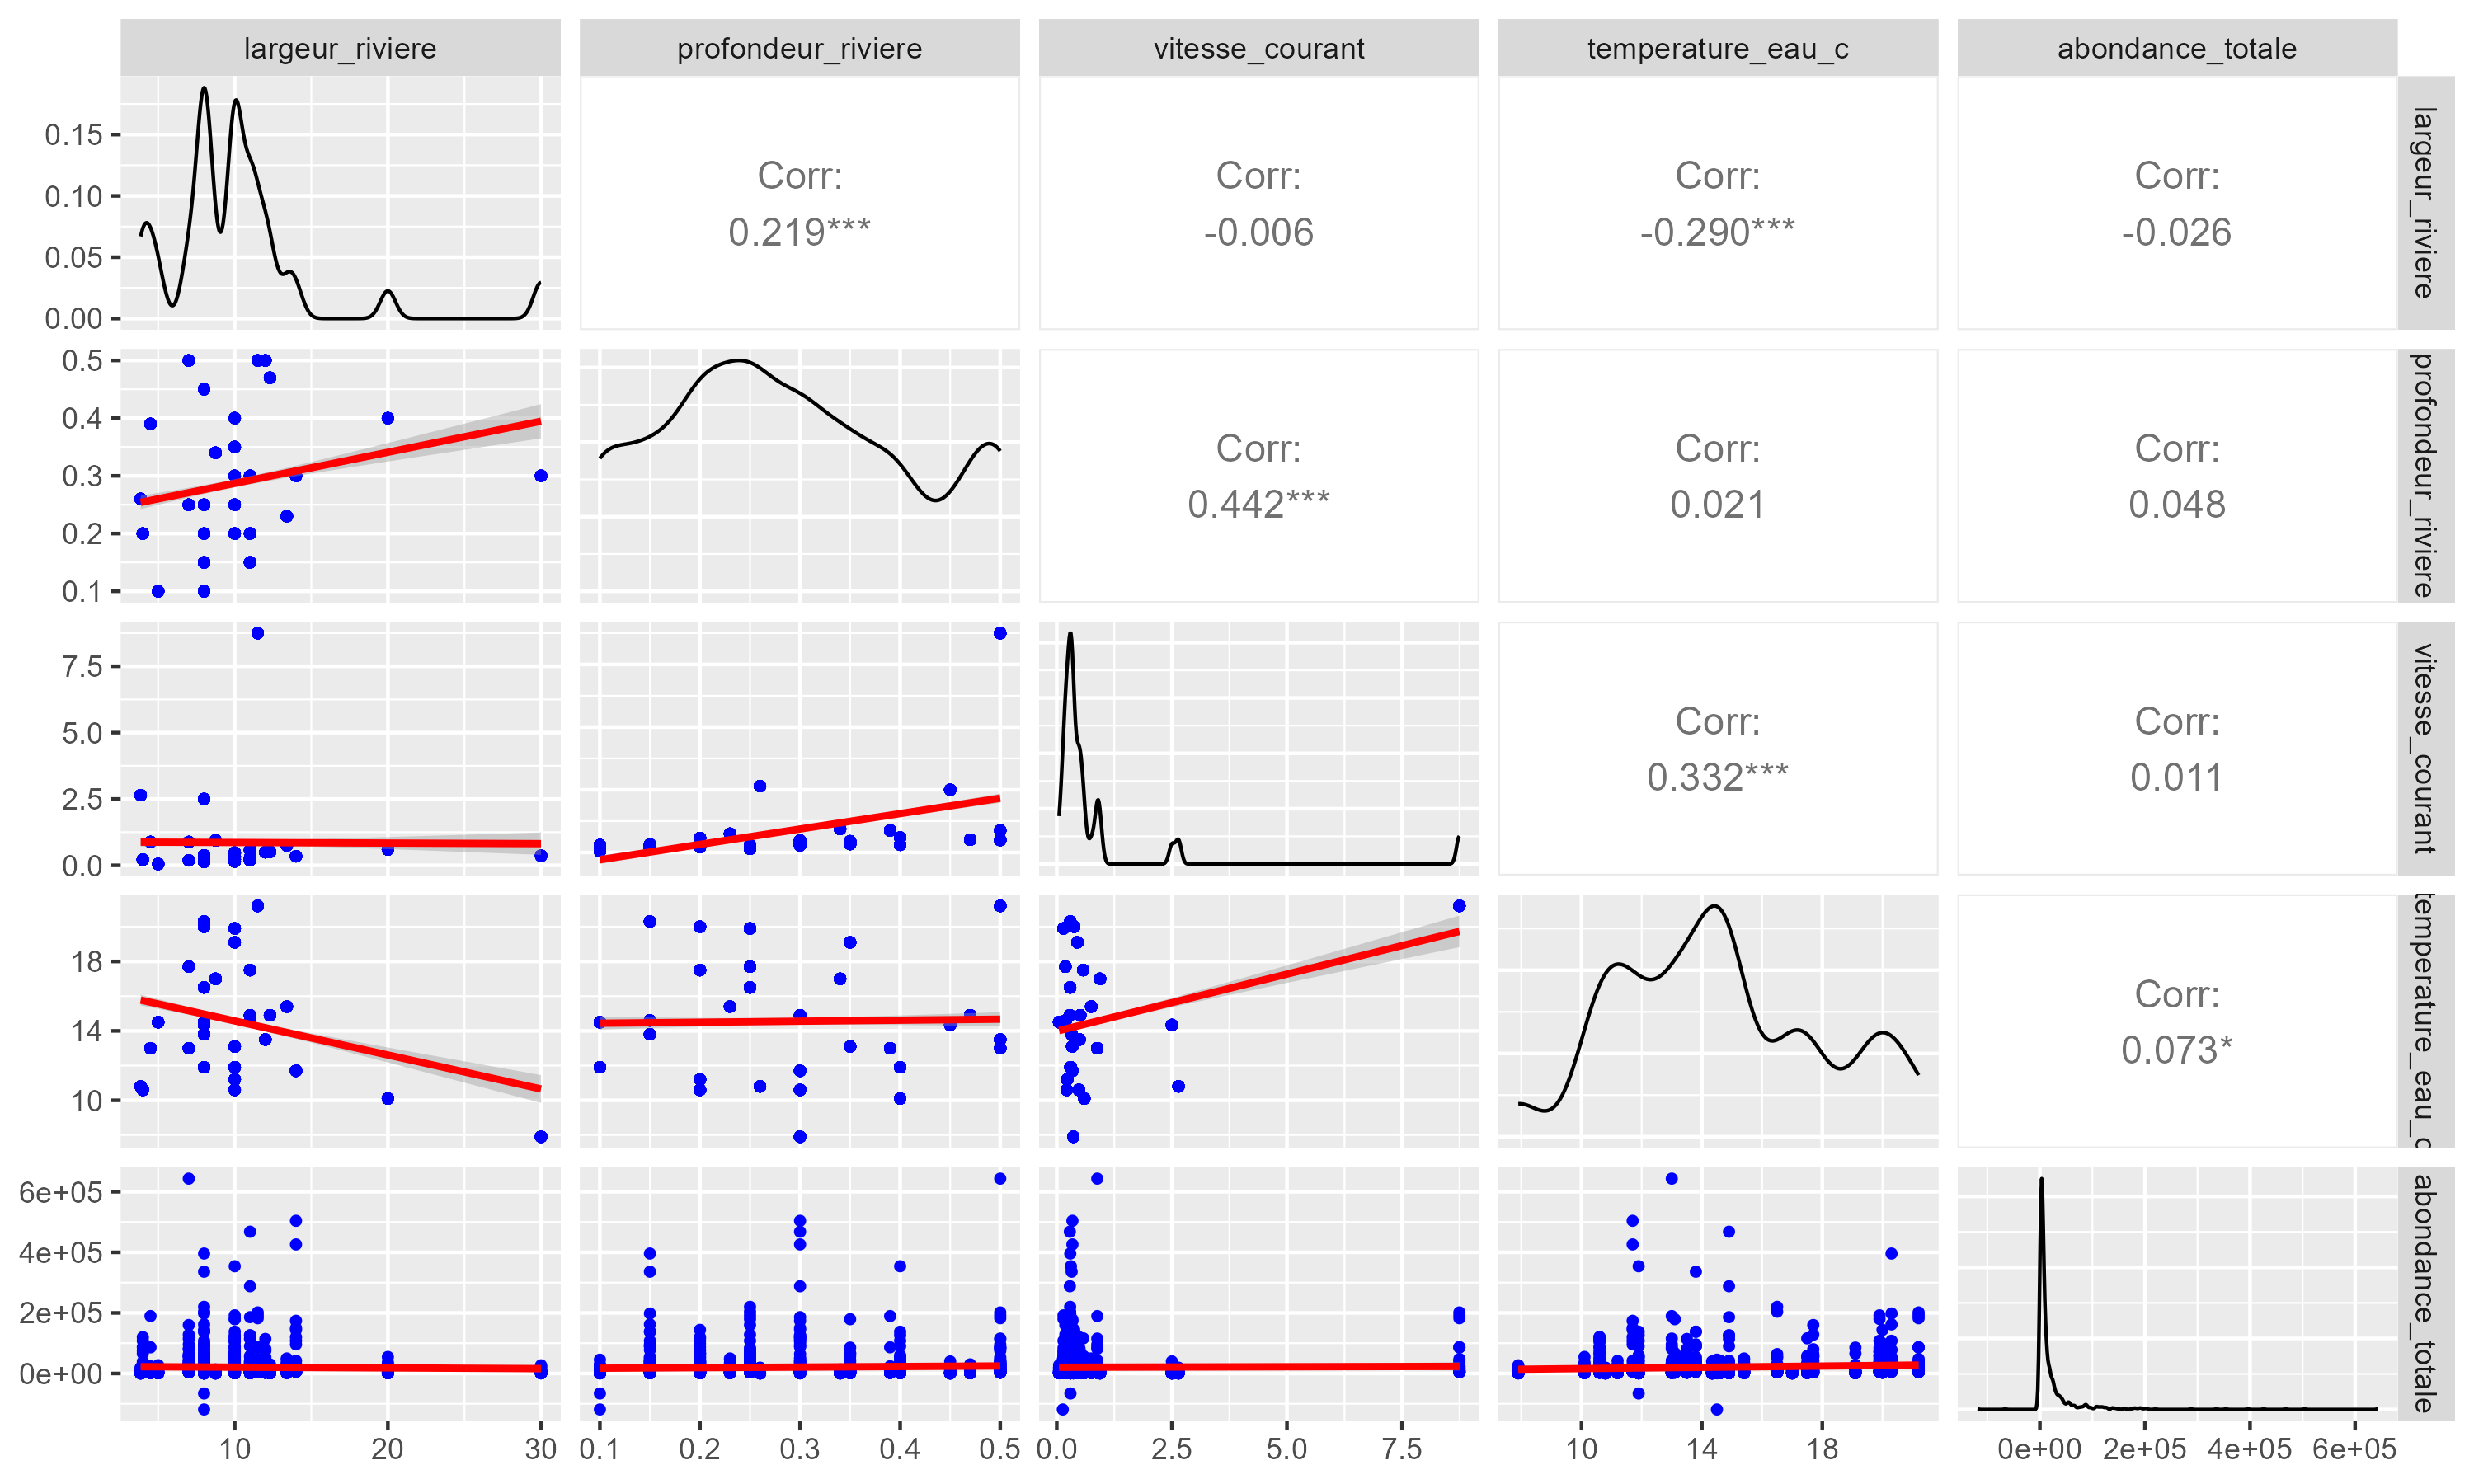
\includegraphics[width=0.5\textwidth,height=0.26\textheight]{"C:/Users/ALEXIS/OneDrive/Bureau/Atelier2_ AlexisGabJust/projet-gab-alex-just/figure_3.png"}
\caption{Corrélation entre paramètres physiques des rivières et
abondance des macro-invertébrés benthiques, avec diagrammes de
dispersion et densité. \label{fig:plot1}}
\end{figure}

\begin{figure}
\centering
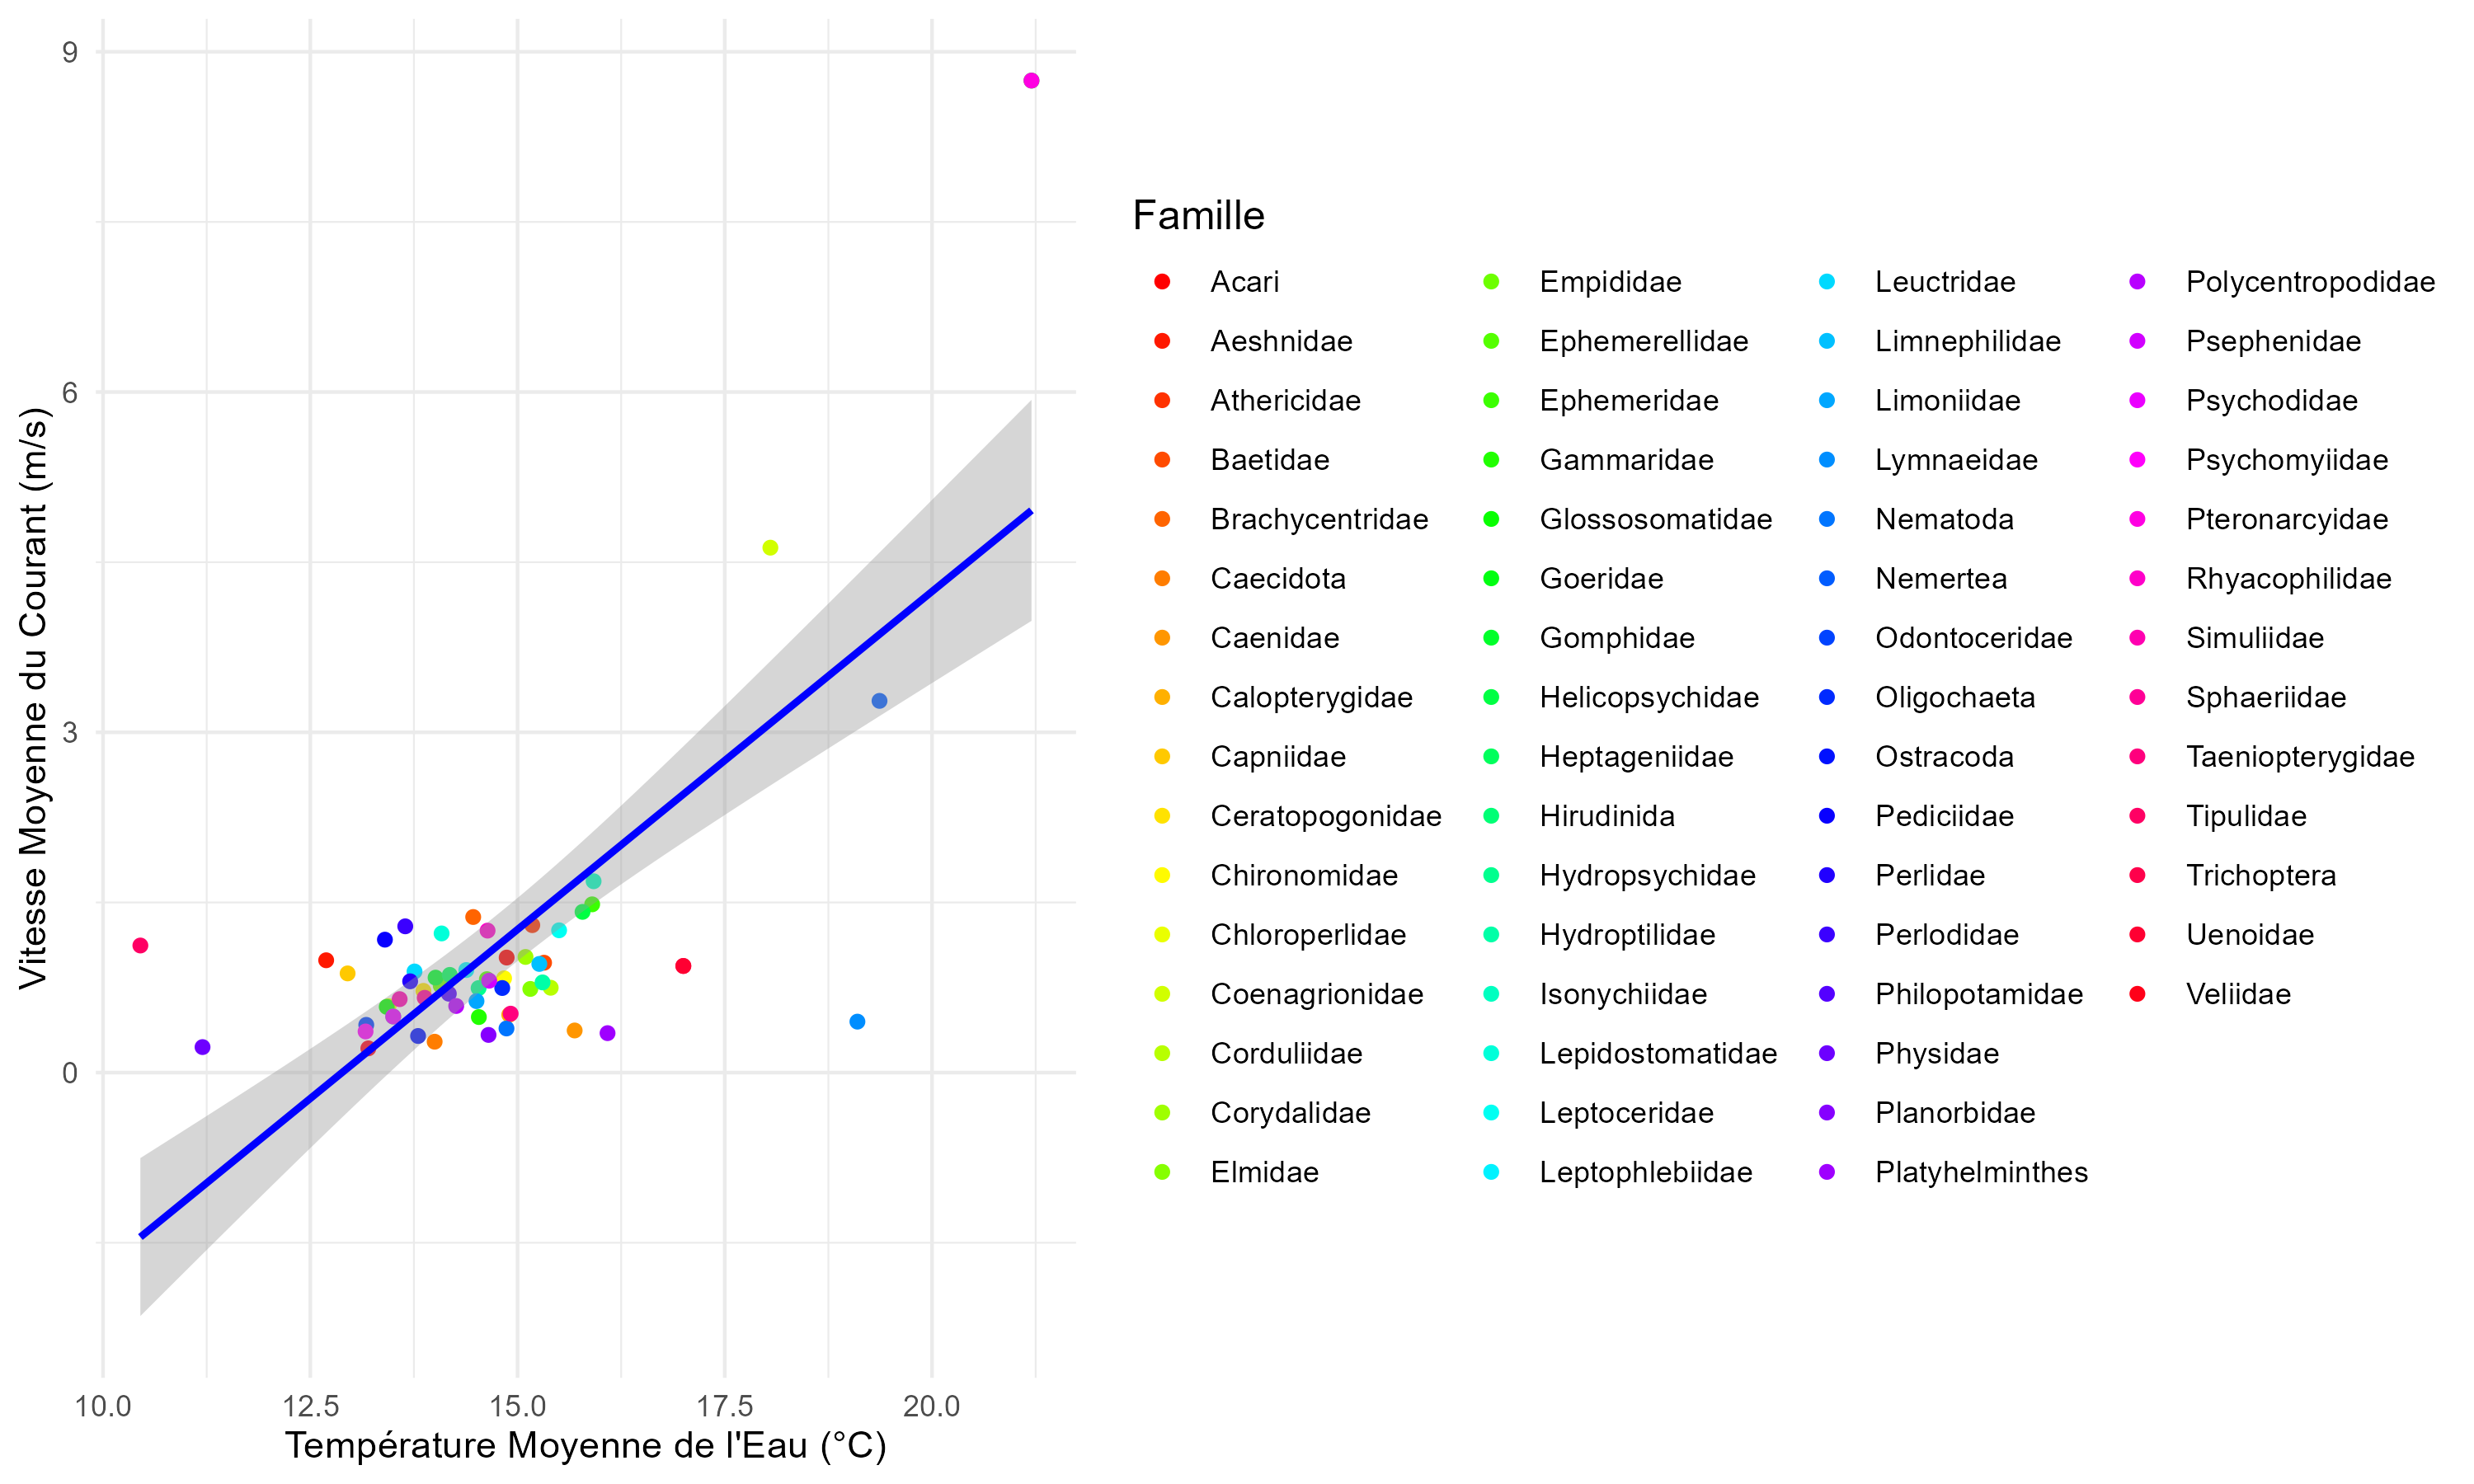
\includegraphics[width=0.5\textwidth,height=0.26\textheight]{"C:/Users/ALEXIS/OneDrive/Bureau/Atelier2_ AlexisGabJust/projet-gab-alex-just/figure_1.png"}
\caption{Relation entre la vitesse moyenne du courant et la température
moyenne du cours d'eau avec la position des taxons associés.
\label{fig:plot1}}
\end{figure}

\begin{figure}
\centering
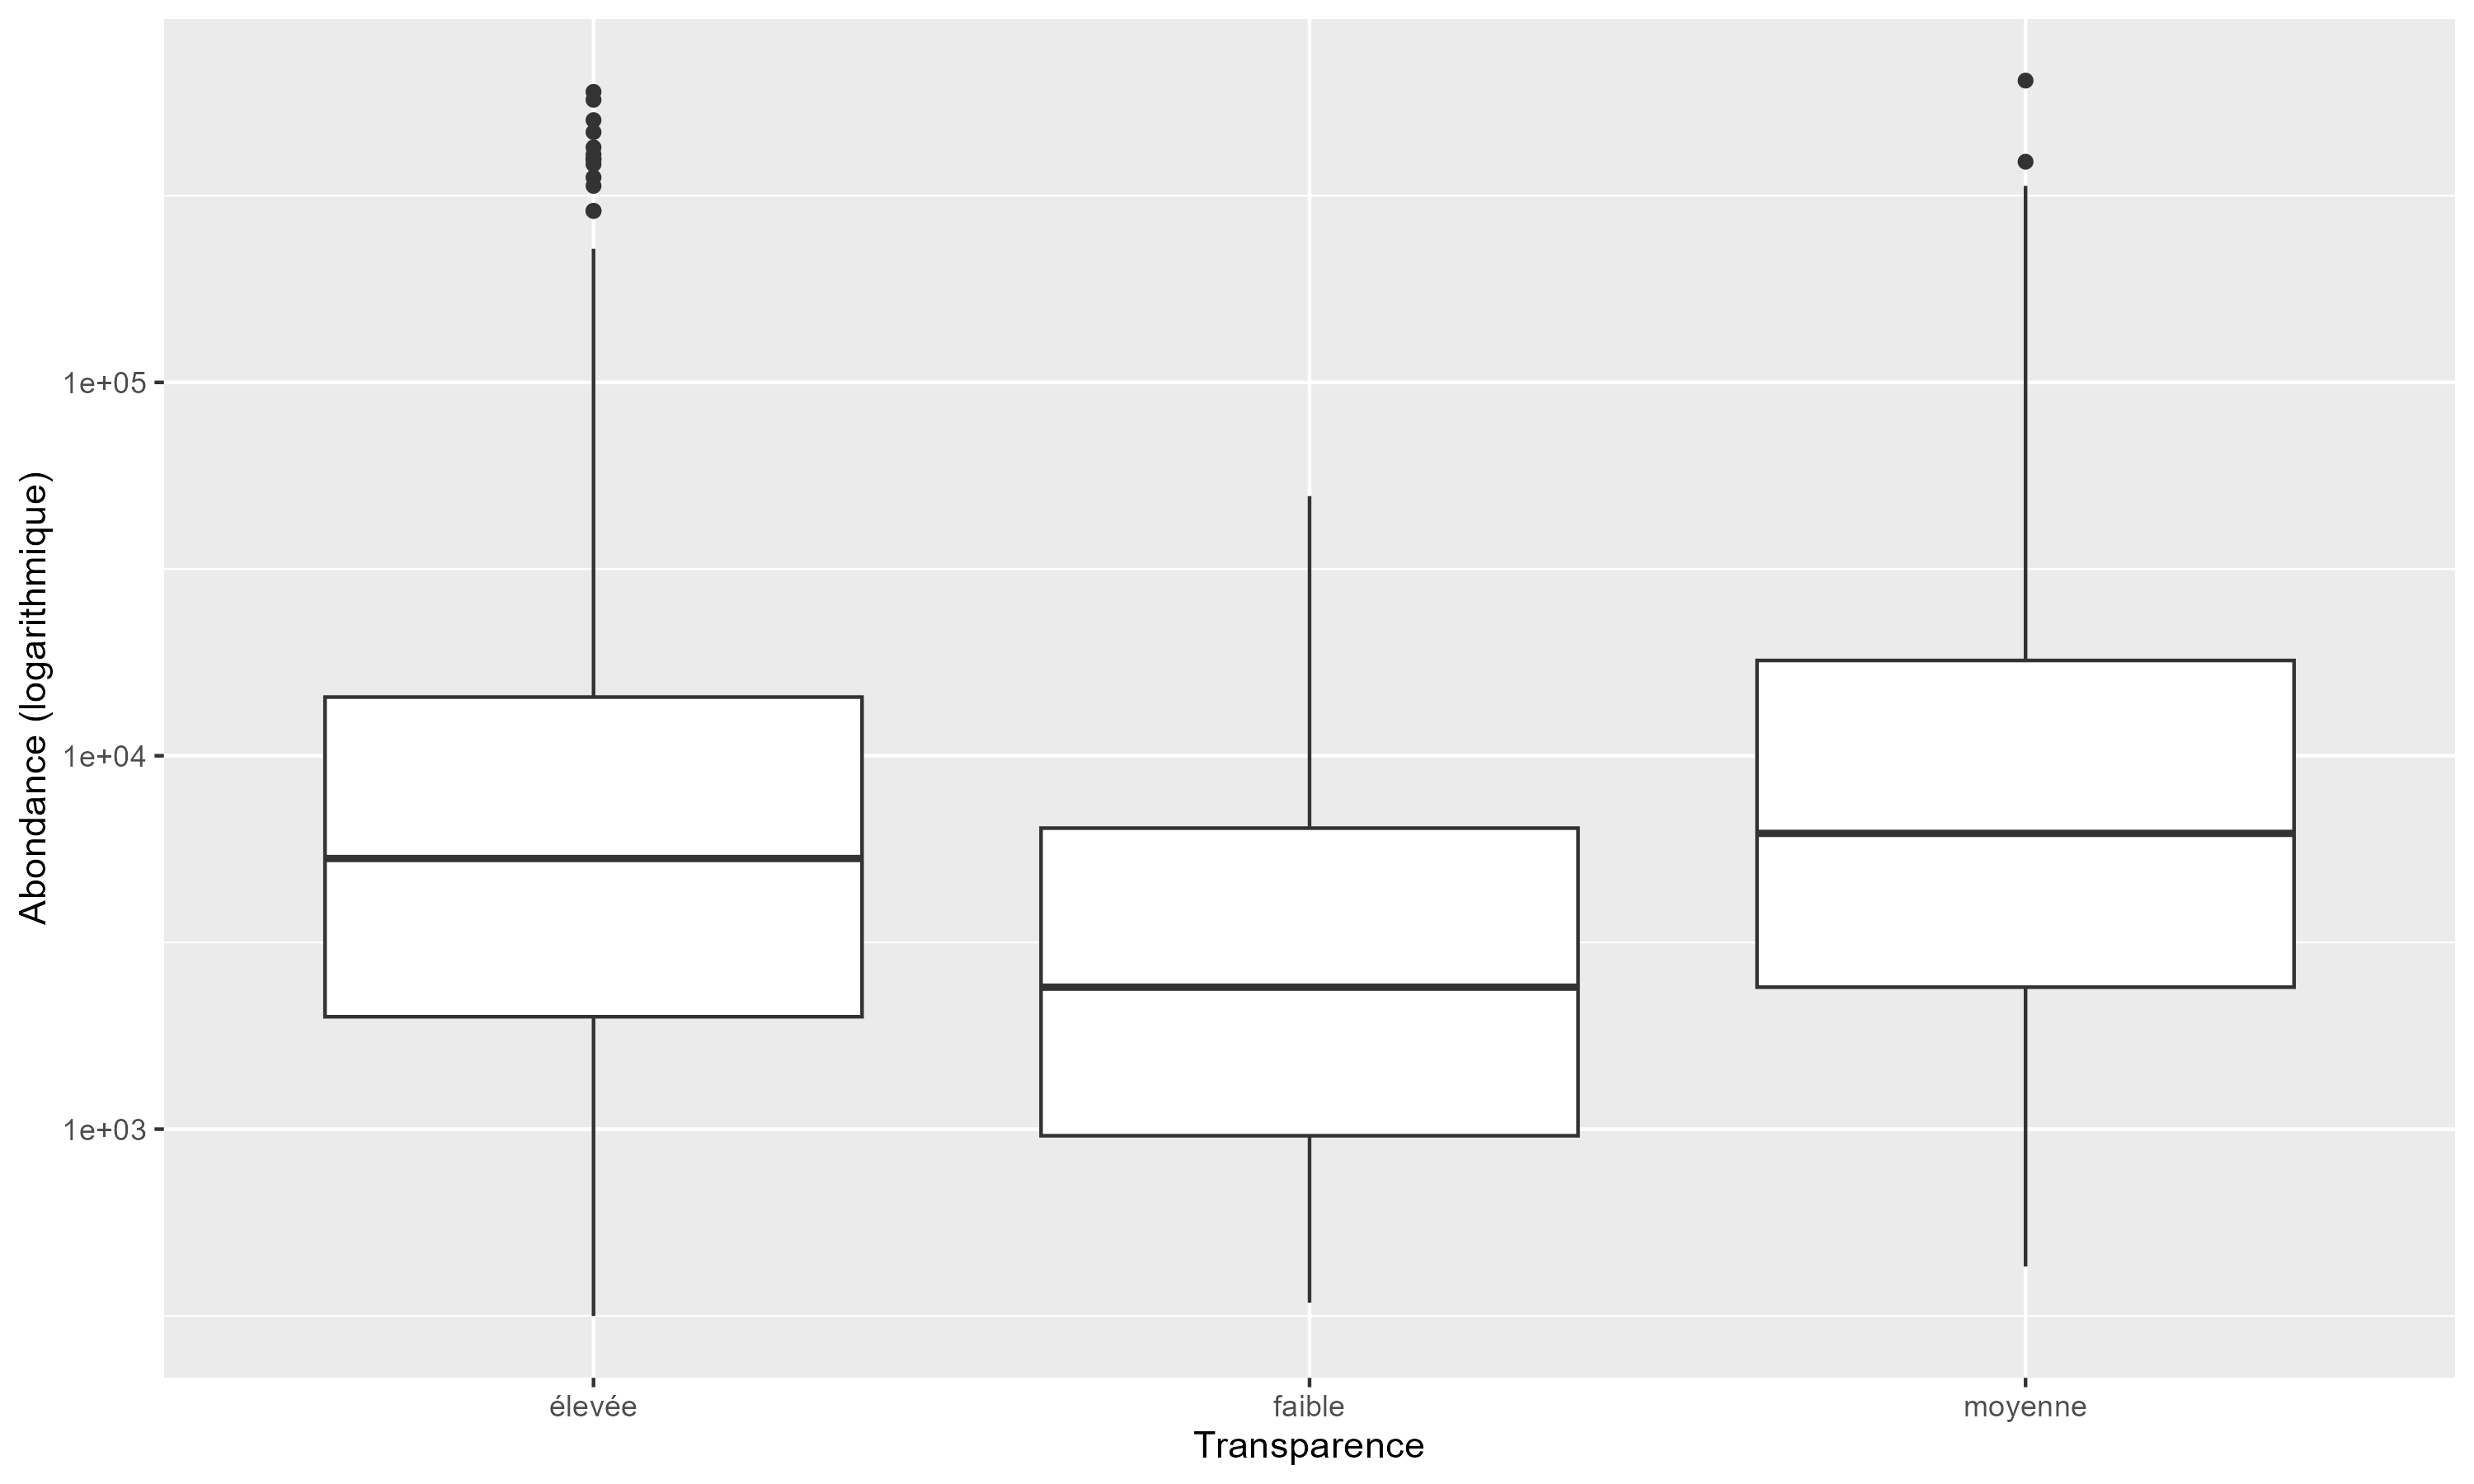
\includegraphics[width=0.5\textwidth,height=0.26\textheight]{"C:/Users/ALEXIS/OneDrive/Bureau/Atelier2_ AlexisGabJust/projet-gab-alex-just/figure_2.png"}
\caption{Relation entre la transparence de l'eau (élevée, moyenne et
faible) et l'abondance totale des organismes benthiques .
\label{fig:plot1}}
\end{figure}

\hypertarget{Discussion}{%
\subsection*{Discussion}\label{Discussion}}
\addcontentsline{toc}{subsection}{Discussion}

La matrice de corrélation présentée à la figure 1 fournit une vue
d'ensemble des relations potentielles entre les paramètres physiques des
rivières soit la profondeur (m), la largeur (m), la vitesse du courant
(m/s) et la température de l'eau (°C). Nous souhaitions observer des
corrélations entre ces différentes caractéristiques et l'abondance
totale des organismes benthiques. Les corrélations significatives dans
la figure 1 sont en accord avec les résultats retrouvés dans la
littérature scientifique. En effet, des études antérieures montrent
souvent une corrélation positive entre l'abondance du benthos et la
température de l'eau qui peut affecter leur métabolisme, leur taux de
croissance ainsi que leur reproduction (2, 3). Ces résultats nous
montrent que, bien que certaines relations entre les caractéristiques
physiques des rivières et l'abondance benthique ne soient pas
significatives, d'autres, telles que la température de l'eau, peuvent
avoir un impact, bien que faible, sur l'abondance du benthos dans les
rivières. Il est important de comprendre que ces corrélations
n'impliquent pas nécessairement une relation de cause à effet et que des
analyses plus approfondies seraient nécessaires pour démystifier les
interactions complexes au sein de ces écosystèmes aquatiques.

L'interprétation écologique de la figure 2 lie la transparence de l'eau,
indice de sa qualité, à l'abondance du benthos. Une eau claire,
indiquant peu de particules en suspension, laisse pénétrer davantage de
lumière, stimulant la photosynthèse et la productivité primaire,
bénéficiant ainsi à la chaîne alimentaire disponible pour les organismes
benthiques. À l'inverse, une eau trouble, avec une faible transparence
due à une turbidité élevée, limite l'exposition à la lumière et peut
réduire la disponibilité alimentaire pour le benthos. La présence de
variations significatives dans les données suggère l'influence d'autres
facteurs environnementaux, indiquant des interactions écologiques
complexes influençant les organismes benthiques. Les écarts importants
et valeurs aberrantes dans les données nécessitent une exploration plus
approfondie, et des analyses statistiques supplémentaires pourraient
clarifier les mécanismes sous-jacents. Les avis scientifiques divergent
; l'étude de Lunt et Smee révèle que la turbidité peut favoriser une
plus grande abondance benthique en offrant un refuge contre les
prédateurs (4). Tandis que Norton note que la prédation est plus élevée
dans les eaux claires, réduisant ainsi l'abondance benthique (5).
Cependant, l'étude de Bigham a eu du mal à démontrer des liens
significatifs entre la turbidité et les communautés benthiques en raison
de réponses variables entre différentes familles, soulignant le besoin
de recherches futures pour des conclusions définitives (6).

L'objectif de la figure 3 était de déterminer l'influence de la
température sur la vélocité des cours d'eau, tout en explorant les
potentiels variations de cette influence sur différents taxons
benthiques. Ainsi, la tendance positive qui émerge de l'analyse,
suggérant une augmentation de la vitesse du courant en relation avec
l'élévation de la température, est une conséquence probable de la
réduction de la densité de l'eau chaude, ce qui diminue la friction et
favorise un écoulement plus aisé de l'eau. L'hétérogénéité des points de
données révèle que les taxons de macro-invertébrés montrent des vitesses
de courant variables à des températures identiques, reflétant des
préférences écologiques ou des tolérances spécifiques aux gradients de
température et de courant. Par exemple, des organismes tels que certains
Trichoptères, qui nécessitent des eaux calmes et des substrats stables
pour s'accrocher ou ériger des habitats (7), contrastent avec des taxons
comme les Pteronarcyidae, qui prospèrent dans des courants plus vifs,
favorables à leur oxygénation et à l'apport en nutriments (8). En outre,
la température est un facteur déterminant du métabolisme benthique,
influençant la croissance, la reproduction et la survie. Les
températures accrues peuvent stimuler ces processus jusqu'à une limite,
au-delà de laquelle les conditions deviennent hostiles (9, 10). Ainsi,
la distribution des données peut être interprétée comme une cartographie
des niches écologiques favorables à chaque taxons, délimitées par des
seuils de températures critiques.

\hypertarget{Conclusion}{%
\subsection*{Conclusion}\label{Conclusion}}
\addcontentsline{toc}{subsection}{Conclusion}

En conclusion, le graphique met en lumière la complexité des
interactions entre les paramètres abiotiques et la biodiversité
benthique, soulignant l'importance de la température et de la dynamique
hydraulique dans la structuration des communautés aquatiques. Ces
observations forment la base d'une compréhension plus approfondie des
écosystèmes fluviaux, offrant des perspectives essentielles pour la
conservation et la gestion des ressources aquatiques.

\showmatmethods
\showacknow
\pnasbreak

\hypertarget{refs}{}
\begin{CSLReferences}{0}{0}
\leavevmode\vadjust pre{\hypertarget{ref-sinokrot_-stream_2000}{}}%
\CSLLeftMargin{1. }%
\CSLRightInline{Sinokrot BA, Gulliver JS (2000)
\href{https://doi.org/10.1080/00221680009498315}{In-stream flow impact
on river water temperatures}. \emph{Journal of Hydraulic Research}
38(5):339--349.}

\leavevmode\vadjust pre{\hypertarget{ref-lenat_effects_1994}{}}%
\CSLLeftMargin{2. }%
\CSLRightInline{Lenat DR, Crawford JK (1994)
\href{https://doi.org/10.1007/BF00021291}{Effects of land use on water
quality and aquatic biota of three {North} {Carolina} {Piedmont}
streams}. \emph{Hydrobiologia} 294(3):185--199.}

\leavevmode\vadjust pre{\hypertarget{ref-paul_streams_2001}{}}%
\CSLLeftMargin{3. }%
\CSLRightInline{Paul MJ, Meyer JL (2001)
\href{https://doi.org/10.1146/annurev.ecolsys.32.081501.114040}{Streams
in the {Urban} {Landscape}}. \emph{Annual Review of Ecology, Evolution,
and Systematics} 32(Volume 32, 2001):333--365.}

\leavevmode\vadjust pre{\hypertarget{ref-lunt_turbidity_2020}{}}%
\CSLLeftMargin{4. }%
\CSLRightInline{Lunt J, Smee DL (2020)
\href{https://doi.org/10.1093/icesjms/fsz214}{Turbidity alters estuarine
biodiversity and species composition}. \emph{ICES Journal of Marine
Science} 77(1):379--387.}

\leavevmode\vadjust pre{\hypertarget{ref-norton_crystal_2023}{}}%
\CSLLeftMargin{5. }%
\CSLRightInline{Norton S (2023) Crystal {Clear} {Problems}: {Impacts} of
{Water} {Transparency} in {Aquatic} {Ecosystems}. \emph{Environmental
Monitor}. Available at:
\url{https://www.fondriest.com/news/crystal-clear-problems-impacts-of-water-transparency-in-aquatic-ecosystems.htm}
{[}Accessed April 24, 2024{]}.}

\leavevmode\vadjust pre{\hypertarget{ref-bigham_review_2021}{}}%
\CSLLeftMargin{6. }%
\CSLRightInline{Bigham KT, Rowden AA, Leduc D, Bowden DA (2021)
\href{https://doi.org/10.5194/bg-18-1893-2021}{Review and syntheses:
{Impacts} of turbidity flows on deep-sea benthic communities}.
\emph{Biogeosciences} 18(5):1893--1908.}

\leavevmode\vadjust pre{\hypertarget{ref-mackay_ecological_1979}{}}%
\CSLLeftMargin{7. }%
\CSLRightInline{Mackay RJ, Wiggins GB (1979)
\href{https://doi.org/10.1146/annurev.en.24.010179.001153}{Ecological
{Diversity} in {Trichoptera}}. \emph{Annual Review of Entomology}
24(Volume 24, 1979):185--208.}

\leavevmode\vadjust pre{\hypertarget{ref-stewart_front_1988}{}}%
\CSLLeftMargin{8. }%
\CSLRightInline{Stewart KW, Stark BP (1988) Front {Matter}. \emph{Nymphs
of {North} {American} {Stonefly} {Genera} ({Plecoptera})} (Entomological
Society of America).
doi:\href{https://doi.org/10.4182/GGDW2452.1988.i}{10.4182/GGDW2452.1988.i}.}

\leavevmode\vadjust pre{\hypertarget{ref-portner_physiology_2008}{}}%
\CSLLeftMargin{9. }%
\CSLRightInline{Pörtner HO, Farrell AP (2008)
\href{https://doi.org/10.1126/science.1163156}{Physiology and {Climate}
{Change}}. \emph{Science} 322(5902):690--692.}

\leavevmode\vadjust pre{\hypertarget{ref-portner_ecosystem_2008}{}}%
\CSLLeftMargin{10. }%
\CSLRightInline{Pörtner H-O (2008)
\href{https://doi.org/10.3354/meps07768}{Ecosystem effects of ocean
acidification in times of ocean warming: A physiologist's view}.
\emph{Marine Ecology Progress Series} 373:203--217.}

\end{CSLReferences}



% Bibliography
% \bibliography{pnas-sample}

\end{document}
